
\chapter{The Steganos Project}
\begin{multicols*}{2}
Steganos is the name of the application that implements the algorithms enumerated in the earlier chapters of this paper and is the direct result of the work done by the authors. In this chapter I will present what modern technologies and frameworks went into creating the application, how it is structured from an Object Oriented point of view, how fast it is and how I hope it will expand into the future.

\section{Used technologies}
\subsection{C++}
C++ is one of the lowest high-level computer programming languages. Designed by Bjarne Stroustrup, it first appeared in 1985 as a variation of one of the most popular languages at the time, C. It is one of the most efficient modern languages mainly because it has been designed with performance and flexibility in mind, just like its predecessor. C++ has gained a lot of traction  from big companies like Intel and Microsoft which needed a programming language that could be used for operations ranging from basic kernel functions to highly specialized Object-Oriented projects with Graphical User Interfaces\cite{c++-programmming-language}.

Since its conception, C++ has grew substantially by adding support for generic and functional features to ease the development processes and getting standardized by the International Organization for Standardization probably helped as well because it meant no more obscure variations of the language, allowing programmers to follow only one standard, ending up with even more portability and stability of the applications.

In the modern day, it is used almost everywhere: the kernel of various operating systems, the transaction software used by banks, drones and airplanes, embedded systems such as the Arduino or Raspberry Pi, and now in the Steganos Project as well under the latest approved standard of the language, C++17.

\begin{figure}[H]
    \centering
    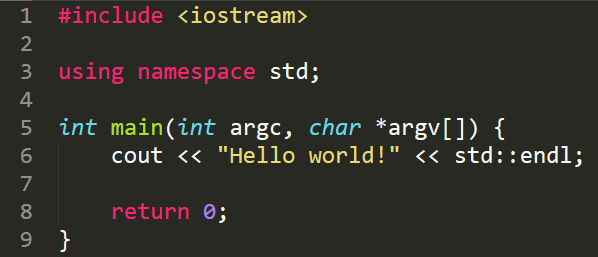
\includegraphics[width=7cm,keepaspectratio]{pics/example_of_cpp_code}
    \caption{Example of C++ code}
\end{figure}

\subsection{CMake}
CMake is a cross-platform open-source tool designed for managing the build process of software based on the C++ programming language. It has been created in the year 2000 and ever since then it stayed compiler-independent using simple configuration files that generate the adequate makefiles to be used in the users environment while building the target project\cite{cmake-documentation}.

CMake uses files called CMakeLists.txt that contain the commands to be used by the internals of the tool in the building process. It is required that one file is in the root of the project before running the CMake process, with the possibility of adding a .txt file in the subdirectories in order to indicate special cases that require a different approach.



Each command in CMake has the same format: COMMAND (args..). Using this format, users are able to build even the most complex software projects in the form of simple executables, dynamic or static linked libraries, etc. Steganos uses CMake because it is an extremely effective tool in the building process and it allows for separating the logic of the project into distinct modules i.e. the audio module, the image module, the general usage module, and linking them in the end into a simple executable.

\begin{figure}[H]
    \centering
    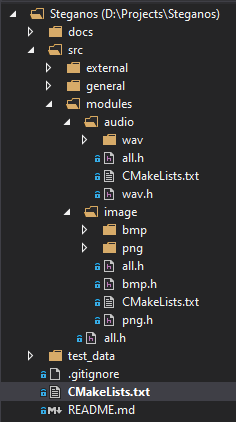
\includegraphics[height=6.9cm,keepaspectratio]{pics/cmake_folder_structure_example}
    \caption{Example of a CMake folder structure}
\end{figure}

\begin{figure}[H]
    \centering
    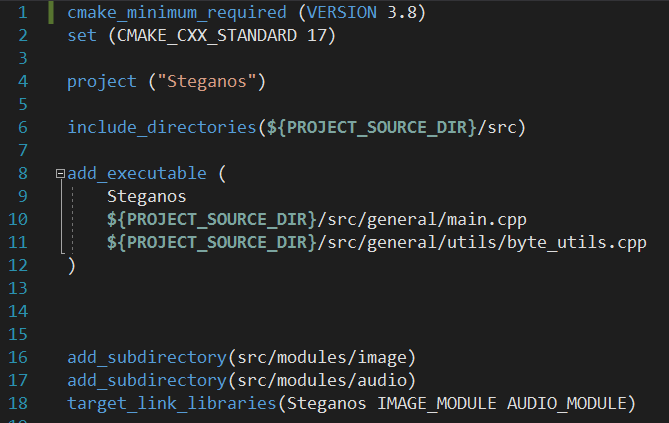
\includegraphics[height=5.2cm,keepaspectratio]{pics/cmake_file_example}
    \caption{Example of a CMakeLists.txt file}
\end{figure}

\subsection{CXXOpts}
\subsection{Lodepng}
\subsection{MMSSTV Engine for Windows}
\subsection{Robot36 for *NIX based systems}

\section{Application architecture}

\section{Benchmarks}

\section{Further work}
\end{multicols*}